%----------------------------------------------------------------------------------------
%  CHAPTER CONTENTS
%----------------------------------------------------------------------------------------

\chapter*{Predicting gender in introductory CS}

\section*{Project Overview}

As I have often said, one of the biggest challenges of this century is successfully getting people into the technical workforce. We are now in the age of automation with autonomous cars driving down our streets and Alexa and Siri becoming an extension of our homes. With the increase of these systems, it is likely that we are also going to see an increase in technical jobs.

This shift in the workforce towards highly skilled, technical knowledge workers poses a challenge on the supply side; mostly because of a lack of presence of computer science in K-12 education; the under-production of post-secondary degrees in computer science;  the underrepresentation of women and the underrepresentation of ethnic minorities.

One of the solutions that have been proffered for this problems is redesigning introductory computer science to broadening participation.  

As part of my doctoral study, I decided to study the socio-curricular factors that affect the decision to participate in introductory computer science through a data-driven lens. To do this, I designed a research study investigating the role of computer science self-identity centered around the experiences of undergraduates in two introductory computer science classes at UC Berkeley.


\section*{Problem Statement}

With this project, the problem I am interested in investigating is the gendered experience of these the two CS classes in my study. Using machine learning algorithms, I want to predict and identify the most salient variables that govern the experience of men versus women in introductory CS at an elite research university like Berkeley.

To predict gender in intro CS at Berkeley we suggest the following strategy:
\begin{enumerate}% 
\item Explore the dataset to ensure its integrity and understand the context.
\item Identify features that may be used. If possible, engineer features that might provide greater discrimination.
\item With the understanding that this a ``classification'' task, explore a couple of classifiers that might be well suited for the problem at hand.
\item Once a classifier has been selected, tune it for optimality.
\end{enumerate}

\section*{Metrics}


Predicting gender in intro CS is a supervised learning problem. To determine the performance of the model, I have selected ``accuracy" as the metric of most interest. In addition to that, we will take a look at the confusion matrix for the output of each model to give us more insight into how good our classifiers are at discriminating the data based on gender. 

%----------------------------------------------------------------------------------------
%  CHAPTER 
%----------------------------------------------------------------------------------------

\chapter*{Analysis}

\section* {Dataset}
This project uses a dataset which I created as part of my doctoral research. The dataset consists of survey responses. A copy of the survey instrument can be found in the appendix of this report \ref{surveyInstrument}. The survey instruments were developed to measure participants' self-reported efficacy along several dimensions. 

\begin{enumerate}% 
\item Self-reported attitudes about CS
\item Gendered belief about CS ability
\item Career driven beliefs about CS
\item Self-reported attitudes about computational thinking
\item Self-reported attitudes about CS class belonging
\item Self-reported beliefs about collegiality
\item Prior collegiate CS exposure
\item CS mentors and role models
\end{enumerate}



Majority of the questionnaire uses a 5-point Likert scale (where 1 = Disagree, 3 = Neutral and 5 = Agree). A code book was created to facilitate ease of analysis and interpretability of results. Using the function \texttt{dataDescr()} gives an introduction to the dataset along with codes and the questions which those code represent. For individual look up of codes, the function \texttt{dataLookUp('atct\_8')} can be used.

The dataset consists of 882 instances with no missing data. Further, there are 494 males and 388 female samples in the dataset.

An interesting aspect of this dataset is that the class labels for our classification are slightly unbalanced at a ratio of around 1:1.2 for male students as can be seen in figure \ref{targetClass}. 

\begin{figure}[!hbtp]
\centering
    \subfloat[]{%
    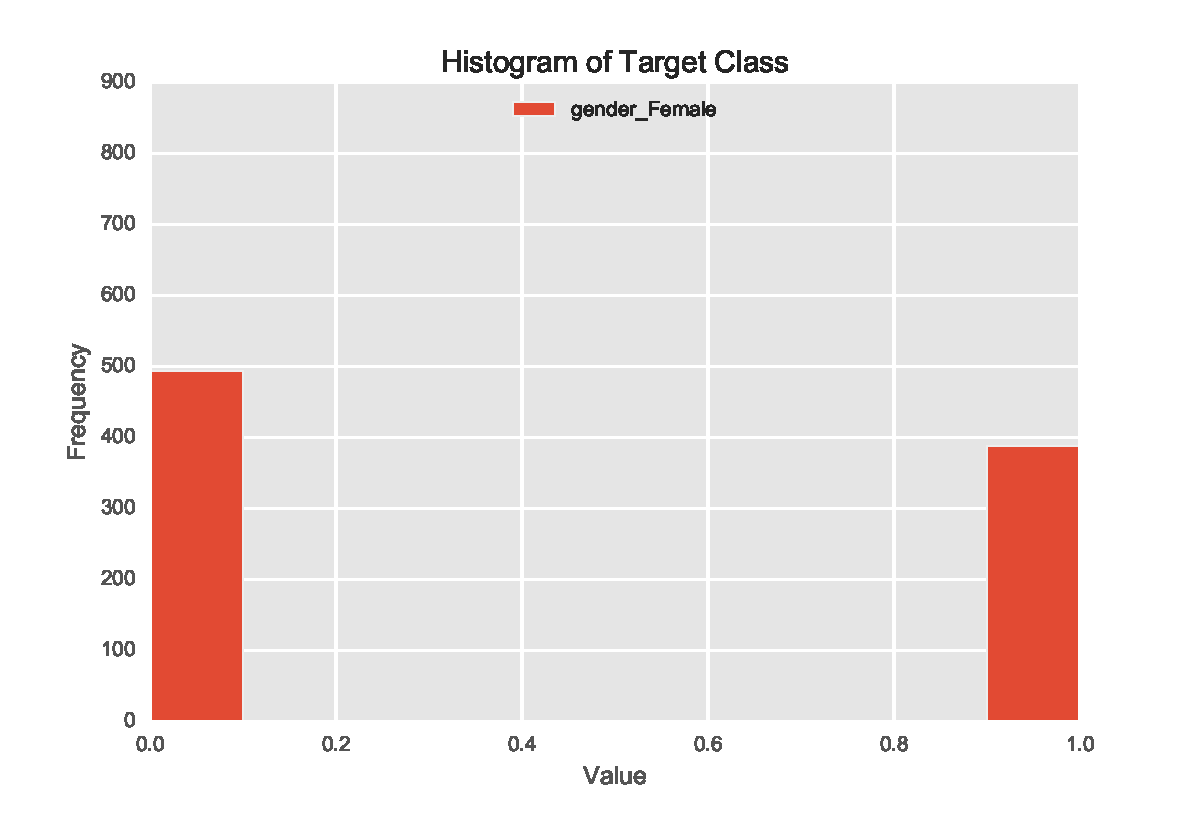
\includegraphics[width=0.8\textwidth]{figures/targetClass}
    \label{targetClass}}
    
    \caption{\textbf{Gender plot. }\textit{The histogram shows a slightly unbalanced target dataset with 494 values of \{0: male\} and 388 values of \{1: female\}.}}
\end{figure}



\section*{Algorithms and Techniques}

For the problem of predicting gender in intro CS I experimented with four different classifiers, a decision tree classifier, two ensemble methods and a support vector machine:

\begin{enumerate}% 
\item A RandomForestClassifier\\
I selected this learner because it is considered one of the best off-the-shelf learning algorithm, and requires almost no tuning. 
\item An eXtreme Gradient Boosted (XGBoost) Trees Classifier\\
XGBoost is an advanced implementation of gradient boosting algorithm. From reading literature on machine learning in practice, the XGBoost classifier has differentiated itself as a classifier that has successfully demonstrated its performance in a wide range of problems from particle physics, to ad click-through rate prediction and so on. For example, ``among the 29 challenge winning solutions published at Kaggle's blog during 2015, 17 solutions used XGBoost.''

\item Support Vector Machine (SVMs)\\
I selected the SVMs because they are very robust classifiers and \textit{more importantly}, they have a method of \textit{biasing} the soft-margin constant, $C$, to correct for class imbalances. 
              
\item Decision Tree Classifier\\
The \textit{major} reason why the decision tree classifier was selected was its interpretability. For this problem domain, it is not just satisfactory to discriminate between male and female students, what learning researchers ultimately want is to gain \textit{insights} into what the salient factors around the experience of intro CS are so they can correct for negative outcomes.

\end{enumerate}

\section*{Benchmark}

This is novel research, as a result, there are no benchmarks we can compare the performance of our classifiers with.


%----------------------------------------------------------------------------------------
%  CHAPTER 
%----------------------------------------------------------------------------------------
\chapter*{Methodology}


\section*{Data Preprocessing}

To prepare our data for classification, we need to devise a scheme to transform all features into numeric data. This dataset as several non-numeric columns that need converting. Many of them are simply \texttt{yes} and \texttt{no}, e.g. \texttt{prcs\_2}. We can reasonably convert these into `1'/`0' (binary) values. For the columns whose values are `Nan', we will convert these to `0'. We removed the spaces from some column names with the understanding that the tree plotting algorithm for Xgboost will fail if column names have spaces. 

We scaled the features using a minimax scaler to get better output for our SVM. This yielded the following values:
\begin {itemize}
\item Disagree = 0.0
\item Somewhat disagree = 0.2
\item Neutral = 0.6
\item Somewhat agree = 0.8
\item Agree = 1.0
\end{itemize} 



\section*{Frequency Distribution}
We created a frequency distribution for some dimensions in our data to see if there are features that have extremely low variability in their distribution. From figures \ref{atct_dimension}, \ref{atcs_dimension}, and \ref{blg_dimension}, we know that these variables are broadly distributed.

\begin{figure}[!hbtp]
\centering
    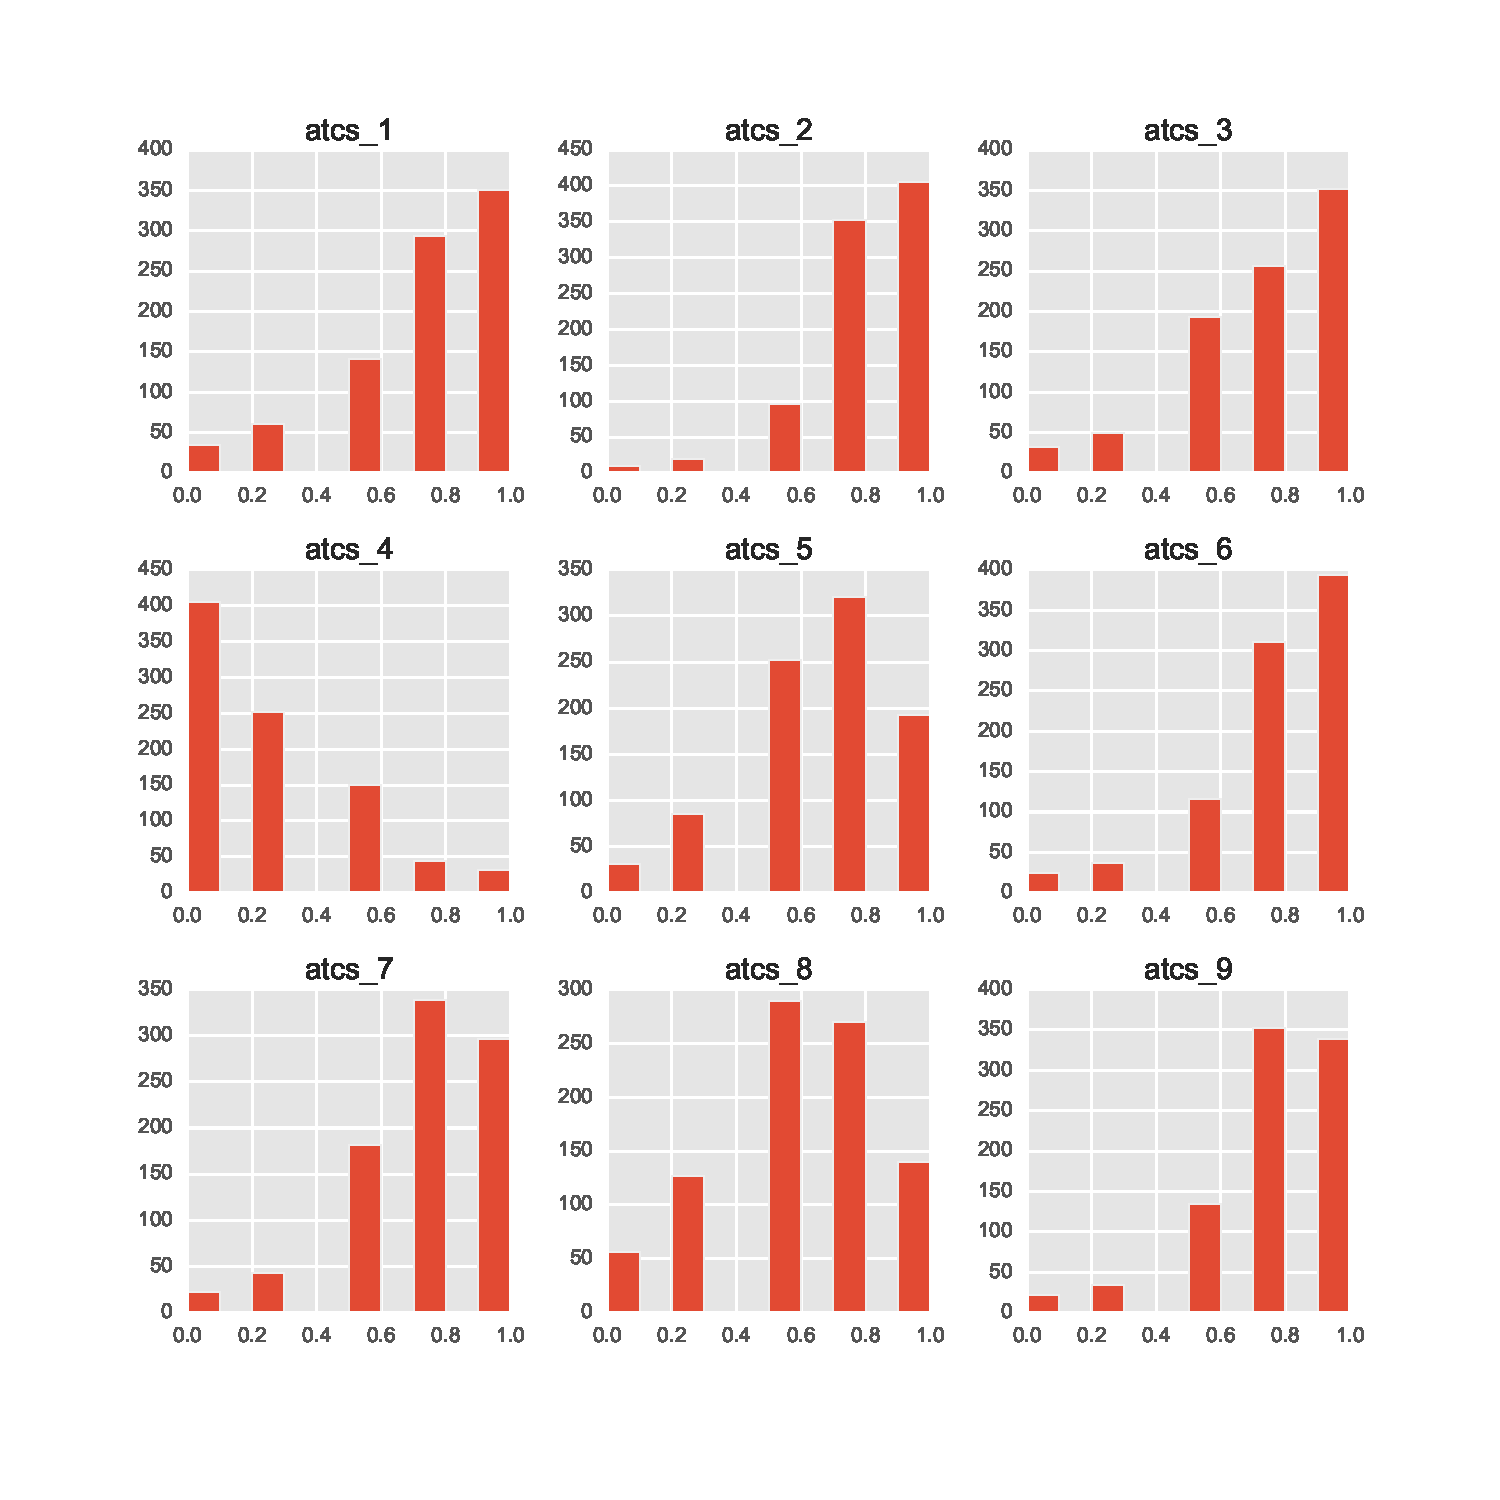
\includegraphics[width=0.8\textwidth]{figures/atcs_dimension}
    \caption{\textbf{Frequency distribution for dimension atcs. }\textit{Self-reported attitudes about CS.}}\label{atcs_dimension}
\end{figure}

\begin{figure}[!hbtp]
\centering

    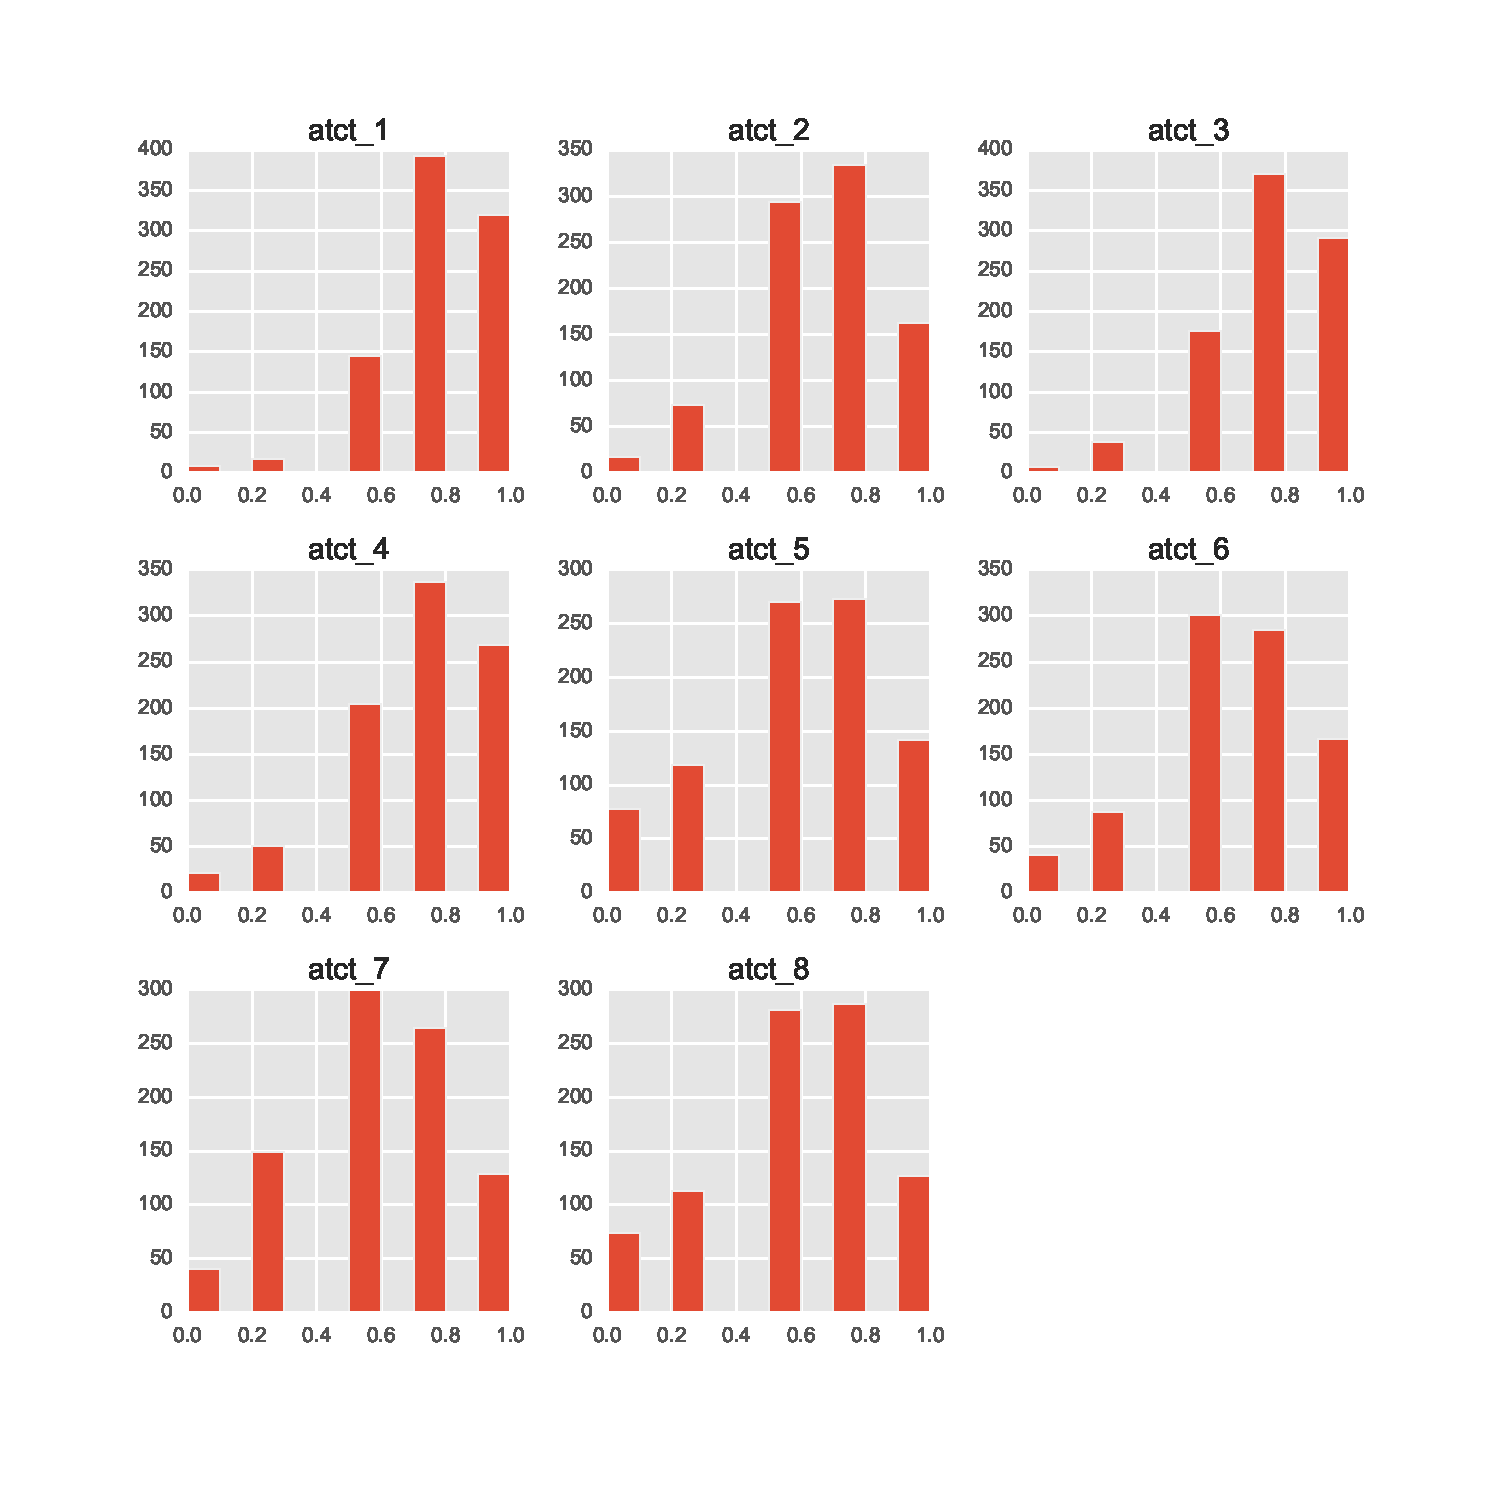
\includegraphics[width=0.8\textwidth]{figures/atct_dimension}
    \caption{\textbf{Frequency distribution for dimension atct. }\textit{Self-reported attitudes about computational thinking.}}\label{atct_dimension}
\end{figure}

\begin{figure}[!hbtp]
\centering
    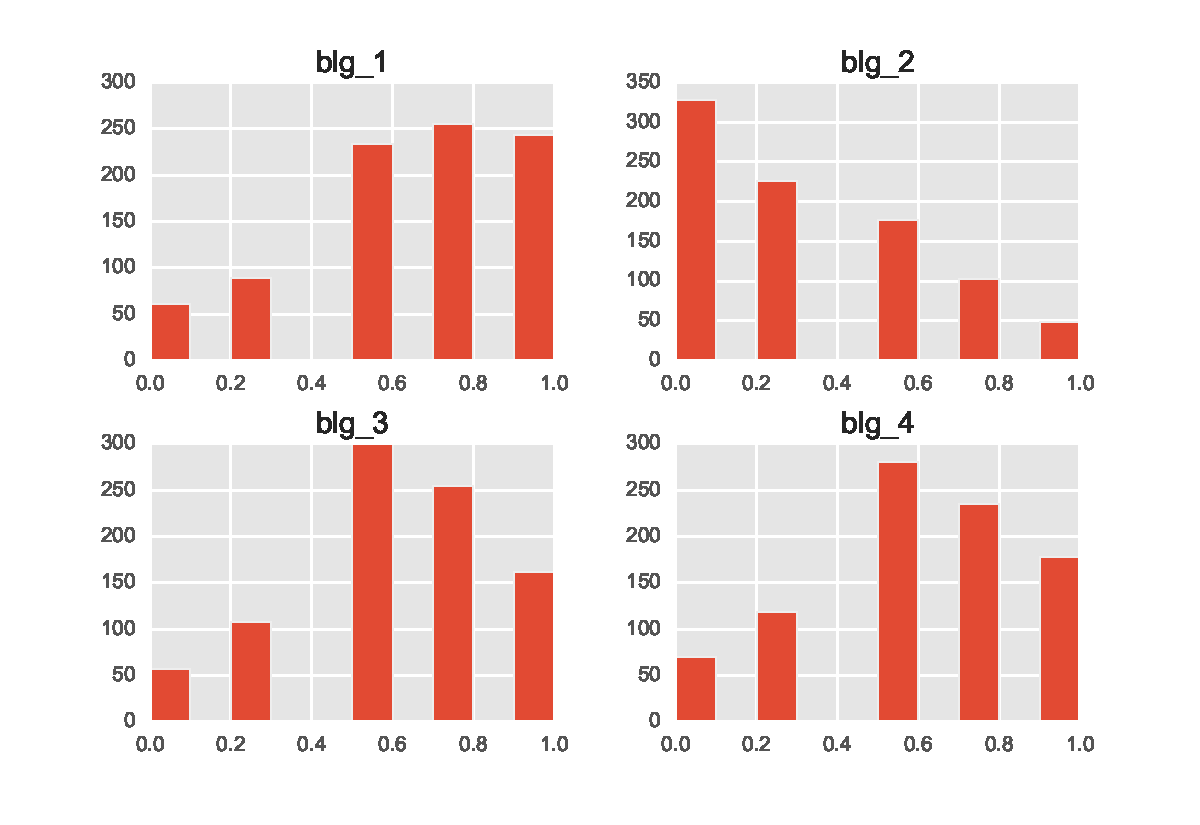
\includegraphics[width=0.8\textwidth]{figures/blg_dimension}
    \caption{\textbf{Frequency distribution for dimension blg. }\textit{Self-reported attitudes about CS class belonging.}}\label{blg_dimension}
\end{figure}

From \ref{atcsgender_dimension}, we can see that the distribution for the dimension \texttt{atcsgender} is extremely skewed to the right, further we notice that \texttt{atcsgender\_2} is bimodal. 

In doing these frequency distributions we are trying to gain an understanding of the variables and determine if we need to reject some of them, or collapse other.


\begin{figure}[!hbtp]
\centering
    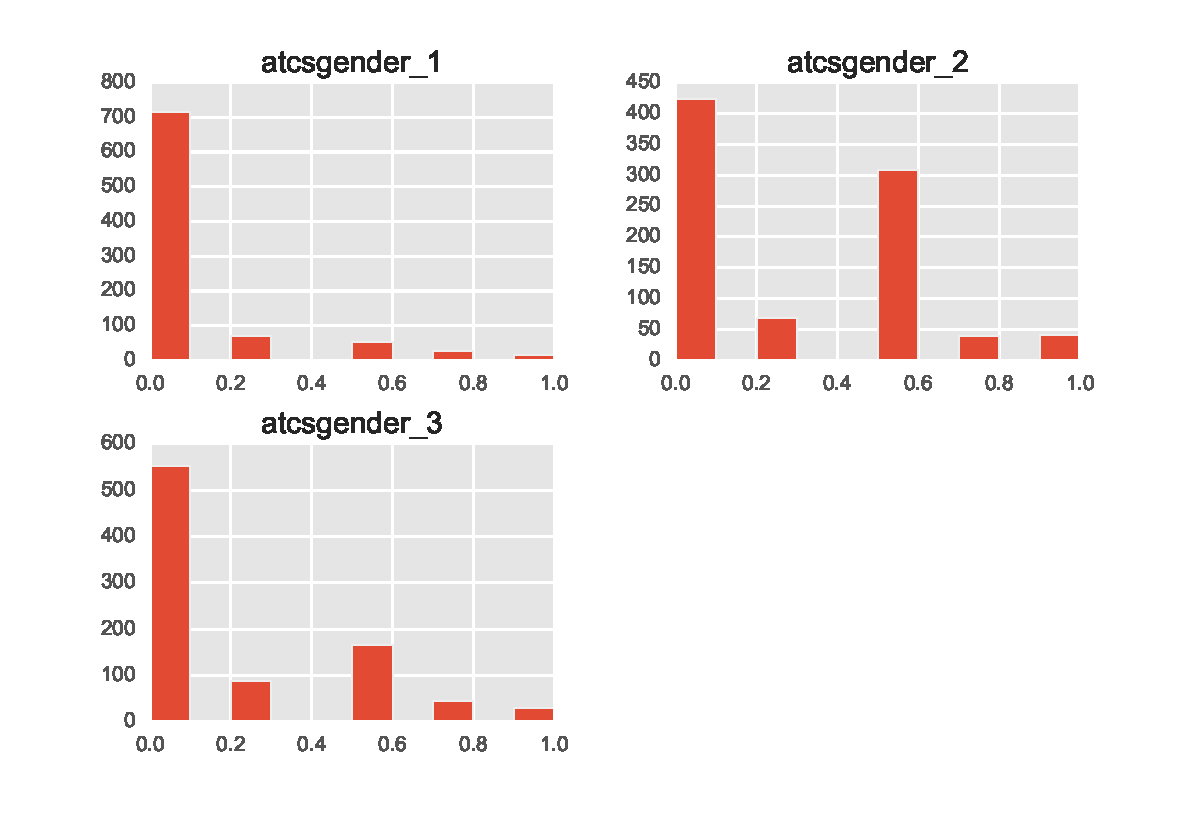
\includegraphics[width=0.8\textwidth]{figures/atcsgender_dimension}
    \caption{\textbf{Frequency distribution for dimension atcsgender. }\textit{Gendered belief about CS ability.}}\label{atcsgender_dimension}
\end{figure}

\section*{Implementation}



\section*{Refinement}

%----------------------------------------------------------------------------------------
%  CHAPTER 
%----------------------------------------------------------------------------------------

\chapter*{Results}


\section*{Model Evaluation and Validation}


\section*{Justification}


%----------------------------------------------------------------------------------------
%  CHAPTER 
%----------------------------------------------------------------------------------------

\chapter*{Conclusion}



\section*{Reflection}


\section*{Improvement}
